\chapter{Estado del arte} 
\label{sec:arte}

\section{Computación en la nube}

\begin{flushright}
\begin{minipage}[b][4cm][t]{11cm}
\begin{flushright}
{\small \emph{Si alguien me pregunta qué es la computación en la nube,}} \vspace{-1pt} \\
{\small \emph{trato de no complicarme con las definiciones.}} \vspace{-1pt} \\
{\small \emph{Les digo que, simplemente, la computación en la nube es una}} \vspace{-1pt}\\
{\small \emph{manera mejor de gestionar su negocio.}} \vspace{1mm}\\
{\footnotesize Marc Benioff,} \vspace{-1.5pt} \\
{\footnotesize fundador y presidente de Salesforce.\phantom{l}}
\end{flushright}
\end{minipage}
\end{flushright}

La computación en la nube es un recurso del que pueden disponer las empresas para cumplir con sus necesidades y objetivos. Especialmente para los pequeños negocios, se trata de una herramienta con gran potencial. Debido al elevado grado de globalización todas las empresas del sector del comercio electrónico deben ser competitivas y proveer incentivos que las hagan más atractivas que sus competidores. La computación en la nube puede ayudar a las empresas a incorporar nuevas funcionalidades en su sitio web o aplicación, obteniendo un valor comercial a partir de ellas \cite{Azad2016ImprovementOE}. 

La computación en la nube se ha establecido en el presente y futuro de la industria de la tecnología de la información, así como de los negocios \cite{Hashem}. Ha revolucionando la industria IT aportando flexibilidad a las organizaciones permitiendo que solo paguen por los recursos y servicios que utilizan y durante su tiempo de uso. 

De forma resumida, la computación en la nube es un tipo de modelo de prestación de servicios, con acceso en cualquier momento y facturación por uso. Su arquitectura tiene las siguientes características básicas:

\begin{itemize}
    \item \textbf{Elasticidad}. La habilidad de escalar hacia arriba o abajo las necesidades de computación según los requisitos del cliente.
    \item \textbf{Conectividad}. Permitir el acceso a los servicios a cualquier hora desde cualquier lugar.
    \item \textbf{Visibilidad}. Ofrecer a los consumidores visión y control de los parámetros de despliegue del servicio, uso y coste
    \item \textbf{Uso compartido}. La habilidad de compartir almacenamiento físico, memoria y red en el mismo espacio físico para diferentes usuarios.
    \item \textbf{Medición del servicio}. Medir el servicio y establecer la factura según esos parámetros.
\end{itemize}

La computación en la nube posee una serie de características positivas para hacer frente al rápido crecimiento de las economías y barreras tecnológicas. Permite a las organizaciones centrarse en el negocio principal sin preocuparse por otros problemas como pueden ser la infraestructura, la flexibilidad y la disponibilidad de recursos.

Los modelos de servicio de computación en la nube más comunes hoy en día son PaaS, SaaS, IaaS, CaaS y FaaS. Cada tipo de servicio está dirigido a unos propósitos y consumidores diferentes. A continuación se enumeran cada uno de estos tipos:

\begin{itemize}
    \item \textbf{Infraestructura como servicio (IaaS)}. El proveedor alquila la infraestructura al consumidor, otorgándole casi la totalidad de su control. Es decir, garantiza el acceso del cliente a los recursos de computación (procesador, RAM, disco duro, entre otros) y a las estructuras de red integradas (cortafuegos, routers, seguridad y copias de seguridad). 
    
    Es el cliente quién selecciona los recursos que necesita para satisfacer sus necesidades. Se trata de un servicio muy flexible, ya que, permite al consumidor ampliar o disminuir los recursos contratados de manera rápida y sencilla siempre que lo necesite.
    
    El proveedor por su parte, es el responsable de garantizar la fiabilidad y la seguridad del sistema, a través del mantenimiento de la infraestructura. El modelo de facturación de este servicio es el pago por uso.
    
    Por tanto, se trata de una herramienta que ofrece grandes ventajas por la desaparición de los costes relacionados con la compra y mantenimiento de hardware. 
    
    \item \textbf{Software como servicio (SaaS)}. También conocido como software bajo demanda, se trata de un servicio que pone a disposición del cliente una aplicación específica lista para ser usada, sin precisar instalación, despliegue o mantenimiento alguno. 
    
    Los usuarios acceden a dicho software a través de un navegador web. Todo está administrado por el proveedor: aplicación, sistema, datos, middleware, sistema operativo, virtualización, almacenamiento y redes. El usuario o bien contrata el servicio o accede a él gratuitamente y hace uso del mismo.
    
    \item \textbf{Plataforma como servicio (PaaS)}. Proporciona un entorno de desarrollo e implementación completo en la nube que permite a los desarrolladores crear aplicaciones y servicios. El consumidor adquiere los recursos que necesita y accede a ellos a través de Internet, pagando tan sólo por el uso que hace de los mismos.
    
    Del mismo modo que IaaS, PaaS también incluye la infraestructura, pero además ofrece otras funcionalidades: middleware, servicios de  inteligencia de negocio, herramientas de diseño y desarrollo, sistemas de gestión de bases de datos, entre otras. PaaS permite a los desarrolladores centrarse únicamente en su trabajo, ya que, soporta todo el ciclo de vida de las aplicaciones web: implementación, compilación, pruebas, administración y actualización.
    
    \item \textbf{Función como servicio (FaaS)}. También conocido como arquitectura \textit{serverless}. Por este término se entiende que las tareas relacionadas con el aprovisionamiento y la gestión de la infraestructura son invisibles para el desarrollador, pero es importante destacar que los servidores siguen existiendo y ejecutando el código.
    
    Las aplicaciones se ejecutan en contenedores sin estado, que se crean en el instante del despliegue y se escalan de forma dinámica, es decir, cuando la demanda disminuye se reduce de forma automática la aplicación.
    
    Este tipo de arquitectura favorece el desarrollo de aplicaciones basadas en microservicios, facilitando el ciclo de vida y la implementación continua. 
    
    \item \textbf{Contenedor como servicio (CaaS)}. Se trata de un servicio intermedio entre el IaaS y el PaaS. Consiste  en un modelo de servicios en la nube que permite a los usuarios implementar y gestionar aplicaciones a través de una forma de virtualización basada en contenedores. 
    
    El proveedor ofrece la plataforma en la que se implementan y gestionan los contenedores, automatizando la administración de la infraestructura. 

\end{itemize}

\newpage

A continuación, se resumen gráficamente las diferencias entre los tipos de servicios cloud:
\begin{figure}[ht]
	\begin{center}
		\includegraphics[width = 0.95\textwidth]{Figuras/Comparación Cloud Computing.png}
	\end{center}
	\caption{\label{fig:differentCloudComputing} Diferencias entre IaaS, CaaS, PaaS, FaaS y SaaS}
\end{figure}

\section{Comercio electrónico}

\begin{flushright}
\begin{minipage}[b][4cm][t]{11cm}
\begin{flushright}
{\small \emph{Cuanto antes eliminemos la "e" de "e-commerce"}} \vspace{-1pt} \\
{\small \emph{y lo llamemos simplemente comercio, mejor.}} \vspace{-1pt} \\
{\footnotesize Bob Willett,} \vspace{-1.5pt} \\
{\footnotesize expresidente de Best Buy International.\phantom{l}}
\end{flushright}
\end{minipage}
\end{flushright}

\vspace{-1cm}

Se entiende por comercio electrónico las transacciones comerciales realizadas digitalmente entre organizaciones y personas. Suelen implicar transacciones que ocurren a través de Internet, la Web y/o dispositivos móviles. Estas transacciones conllevan un intercambio de valor (por ejemplo, dinero) entre organizaciones o individuos a cambio de productos y servicios. El intercambio de valor es importante puesto que sin éste no se produce comercio.

En algunas ocasiones las publicaciones técnicas se refieren al comercio electrónico como negocio electrónico, aunque en algún contexto pueden usarse ambos términos como si fueran sinónimos, conviene marcar la diferencia entre los dos conceptos. El comercio electrónico implica principalmente transacciones de compra y venta que realiza la empresa. El negocio electrónico tiene un enfoque más amplio, que incluye al comercio electrónico, consiste en cómo las empresas aplican la tecnología digital y los medios para mejorar la competitividad de su organización mediante la optimización de procesos internos con canales online y tradicionales para comercializar y suministrar \cite{DigitalBusiness}.

La mayor parte de los académicos comparten la opinión de que el comercio electrónico puede dividirse según la naturaleza de la relación del mercado en \cite{E-commerce2016}:

\begin{itemize}
    \item \textbf{B2B (Business-to-Business)}. Los negocios se centran en vender a otros negocios. Es la forma más grande de comercio electrónico. Por ejemplo: Go2Paper es un mercado externo independiente que sirve a la industria del papel.
    \item \textbf{B2C (Business-to-Consumer)}. Se trata de la categoría más común y discutida de comercio electrónico, donde negocios online intentan vender sus productos a consumidores individuales. Incluye tanto bienes, servicios y contenido online. El ejemplo más claro de este tipo es Amazon.
    \item \textbf{C2C (Consumer-to-Consumer)}. Una forma de que los consumidores se vendan productos o servicios entre ellos, con la ayuda de una plataforma online como Ebay o Etsy. También se pueden destacar empresas como Airbnb o Uber que proporcionan una plataforma similar para servicios como el alquiler de habitaciones o transporte.
    \item \textbf{M-commerce}. Se trata de utilizar dispositivos móviles para realizar transacciones online. Involucra el uso de redes wireless para la conexión con Internet.
    \item \textbf{Social e-commerce}. Implica la utilización  de  las redes sociales para facilitar la compra y venta en línea de productos y servicios. Facebook es el líder de este tipo de comercio. 
    \item \textbf{Local e-commerce}. Se enfoca en atraer al consumidor en función de su localización geográfica actual. Esta forma de comercio electrónico cobra mucha importancia en la actualidad debido a las restricciones de movilidad que se aplican a los ciudadanos en diferentes países del mundo.
\end{itemize}

La situación actual del comercio electrónico está caracterizada por su vertiente social. El contenido de entretenimiento se ha convertido es una de las mayores fuentes de beneficios y el m-commerce se ha instaurado como una realidad con grandes previsiones de crecimiento. El marketing ha sufrido un cambio de paradigma donde se ha sustituido el antiguo marketing transaccional centrado en qué hacer a los clientes por el nuevo concepto de marketing relacional que pone el acento en qué hacer por los clientes \cite{manualGestion}. Las organizaciones han trasladado su presencia online a las redes sociales como Twitter o Instagram, ya que, la gran cantidad de usuarios de estas plataformas suponen una oportunidad de negocio que no debe ser ignorada. Además, han surgido nuevas empresas que han sabido capitalizar activos no utilizados como automóviles o habitaciones libres, tales como Airbnb o Uber \cite{E-commerce2016}. 

En un estudio que la empresa Cetelem realizó sobre el comercio electrónico en España, cuando Miguel Hernández Granado, director de producto para Lenovo en España y Portugal, fue preguntado por la situación actual del comercio electrónico en España, éste respondió: "De los últimos estudios acerca del tema se desprende la idea general de que el sector del comercio electrónico en España está en el buen camino. Tan solo en 2018, el e-commerce rozó en nuestro país los 40.000 millones de euros, lo que supone un incremento del 29\% en comparación con el año anterior, según datos de la Comisión Nacional de los Mercados y la Competencia. Las previsiones de crecimiento y expectativas son favorables e, incluso, aun cuando se espera un descenso en las ventas con relación al ejercicio anterior. Esta tendencia optimista está claramente auspiciada por la madurez del sector y la cada vez mayor normalización de la compra online por parte de los consumidores. España en los próximos años será uno de los países que más crecimiento en e-commerce tendrá en Europa" \citeW{granado}. 

En la siguiente figura se puede observar el crecimiento que experimentaría, antes del Covid-19, el sector del comercio electrónico en España para 2023:

\begin{figure}[ht]
	\begin{center}
		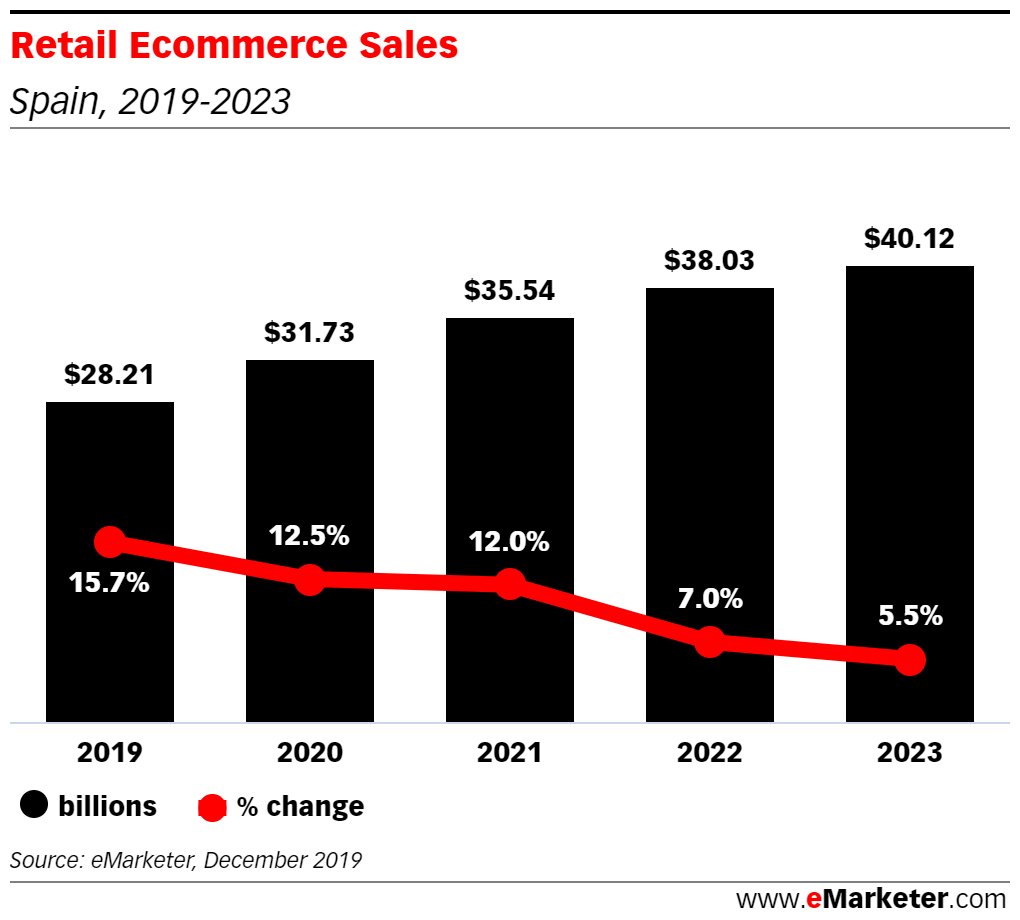
\includegraphics[width = 0.50\textwidth]{Figuras/ecommerce-españa-crecimiento-predicción-.png}
	\end{center}
	\caption{\label{fig:retailSpain} Ventas minoristas de comercio electrónico en España. Fuente: eMarketer.}
\end{figure}

\newpage

La pandemia ha supuesto un duro golpe para el comercio minorista español, se prevee una caída del 12,7\% este año frente a un pronóstico previo de crecimiento del 1,9\%. Sin embargo, ha repercutido positivamente en las previsiones para el comercio electrónico. Se espera que se alcance un total de 32.89 billones de dólares y que continúe aumentando hasta los 41.73 billones en 2023 \citeW{emarketerSpain}. 

Antes de la situación generada por el coronavirus también se esperaba un crecimiento del sector del comercio electrónico a nivel global, como se muestra a continuación:

\begin{figure}[ht]
	\begin{center}
		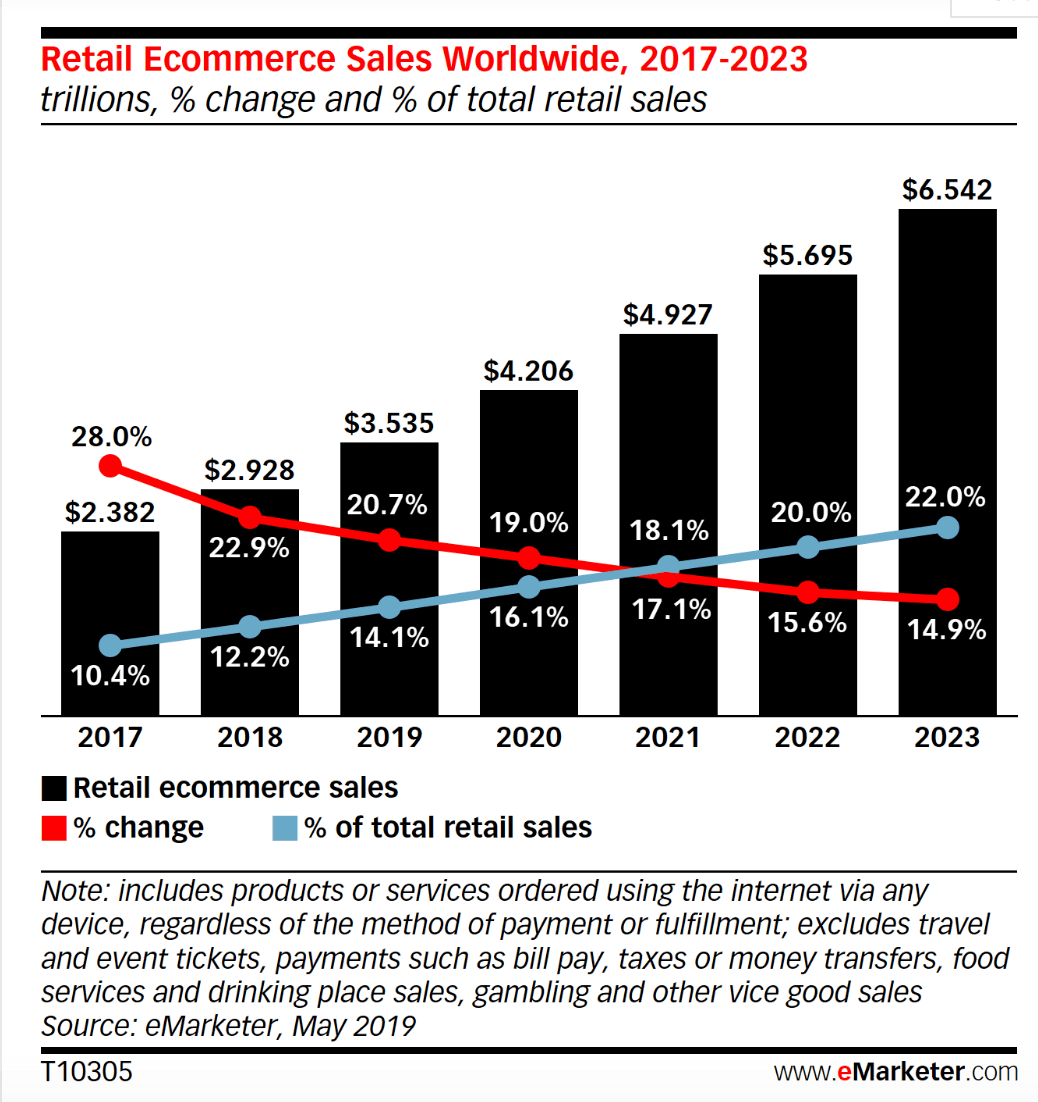
\includegraphics[width = 0.55\textwidth]{Figuras/Global-online-retail-e-commerce-growth.png}
	\end{center}
	\caption{\label{fig:retailWorldwide} Ventas minoristas de comercio electrónico en el mundo. Fuente: eMarketer.}
\end{figure}

A causa de las cuarentenas y los cierres de negocios que están experimentando los consumidores alrededor del mundo, el comercio electrónico se ha convertido en una excelente alternativa de conseguir productos básicos. Este año se espera una tasa de crecimiento  del 16,5\% para el comercio electrónico lo que supone una caída del 3,7\% respecto al pronóstico anterior del 20,2\%. Esta caída será más acentuada en el resto de ventas, un 10\% respecto a las previsiones anteriores \citeW{emarketerGlobal}. 

\newpage

\section{Computación en la nube y comercio electrónico}

La computación en la nube tiene una gran cantidad de connotaciones positivas sobre el comercio electrónico. La ventaja principal es que permite a las empresas reducir en gran medida los costes que supone construir y mantener una página web porque la infraestructura de hardware y software necesaria se puede contratar a un proveedor cloud, pagando tan sólo por el uso que se haga del servicio. Existen otros puntos a favor de esta tecnología \cite{SME}:

\begin{itemize}
    \item \textbf{Escalabilidad}. Se pueden adaptar rápidamente los recursos de los que se hace uso en función de las necesidades del negocio.
    \item \textbf{Disponibilidad y movilidad}. Los usuarios pueden acceder a los productos y servicios de la empresa en cualquier lugar y en cualquier momento. 
    \item \textbf{Foco en el negocio}. Las organizaciones pueden centrarse en la actividad de su negocio y abstraerse de la infraestructura.
    \item \textbf{Administración sencilla}. Convierten el mantenimiento de la infraestructura hardware y software en un proceso más sencillo.
    \item \textbf{Control de desastres}. En el caso de que se produzca un desastre las empresas pueden restablecer su actividad en un período corto de tiempo, ya que toda la infraestructura hardware y software no habrá sufrido daño alguno.
    \item \textbf{Seguridad}. Los proveedores más importantes de servicios cloud garantizan la seguridad de los datos almacenados en sus plataformas.
\end{itemize}

El objetivo último de todas las empresas al adoptar la tecnología cloud es aumentar su competitividad, aunque esta acción por sí misma no garantizará el éxito. Se debe considerar tan sólo como un escalón más en el establecimiento del negocio.

\newpage

\section{Democratización de la IA}

\begin{flushright}
\begin{minipage}[b][4cm][t]{11cm}
\begin{flushright}
{\small \emph{Ya no necesita un presupuesto multimillonario }} \vspace{-1pt} \\
{\small \emph{para introducir la IA en su empresa. }} \vspace{-1pt} \\
{\small \emph{La IA representa una oportunidad para }} \vspace{-1pt} \\
{\small \emph{las empresas más pequeñas de }} \vspace{-1pt} \\
{\small \emph{competir en igualdad de condiciones.}} \vspace{1mm}\\
{\footnotesize Nichole Jordan,} \vspace{-1.5pt} \\
{\footnotesize socio director en Grant Thornton LLP.\phantom{l}}
\end{flushright}
\end{minipage}
\end{flushright}

En un contexto empresarial, se entiende por democratización de la inteligencia artificial hacer que ésta sea accesible para todas las organizaciones. En el pasado siglo se alcanzó una cima de democratización de los recursos tecnológicos, el futuro de la tecnología para las próximas décadas es la Inteligencia Artificial: usar hardware y software para reconocer patrones, hacer predicciones, aprender y mejorar, y tomar medidas basadas en ella. Los más optimistas ven a la IA como una herramienta positiva, que puede ayudar a cada persona a lograr más y mejor.

Gigantes como Google, Amazon, Microsoft, Apple y Facebook son  muy conscientes del poder transformador que conlleva la aplicación de la IA. El aprendizaje profundo es la base del sistema de recomendaciones de Amazon, las herramientas de búsqueda y traducción de Google y el asistente personal Cortana de Microsoft, así como muchas otras aplicaciones y servicios ampliamente utilizados. La mayoría de las empresas que se encuentran entre las 500 más ricas del mundo también tienen equipos dedicados a la IA. El interés de estas grandes fortunas ha agotado los profesionales dedicados a la ciencia de datos, lo que hace especialmente costoso para las pymes la contratación de científicos de datos cuando intentan introducirse en este campo.

Incluso aquellas empresas que pueden permitirse el lujo de contratar a expertos en inteligencia artificial todavía necesitan preparar grandes conjuntos de datos y realizar una fuerte inversión económica en potencia informática para analizarlos y enseñar a su red neuronal a reconocer ciertos patrones u objetos. Sin embargo, los grandes proveedores de la nube se han percatado de los problemas de esta situación y creen que han encontrado una manera de ayudar a las personas a superarlos.

En la actualidad, el aprendizaje automático como servicio, o IA en la nube, se ha convertido en un componente importante de las plataformas como Amazon Web Services (AWS), Microsoft Azure, Google Cloud e IBM Cloud. En esencia, estas compañías ofrecen a sus clientes modelos de aprendizaje profundo previamente entrenados, de modo que puedan ser incorporados por aplicaciones comerciales, por ejemplo, para el reconocimiento de imágenes, así como herramientas que simplifican el proceso de construcción, capacitación y despliegue de modelos personalizados en la nube \citeW{democratizingAI}. 

Con las grandes empresas tecnológicas muy por delante del resto, la industria se pregunta si las pymes realmente pueden beneficiarse de la IA, y transformarse.

\section{Análisis de sentimientos}

\begin{flushright}
\begin{minipage}[b][4cm][t]{11cm}
\begin{flushright}
{\small \emph{Nadie lo expresa así, pero creo que la inteligencia artificial  }} \vspace{-1pt} \\
{\small \emph{es casi una disciplina humanística. }} \vspace{-1pt} \\
{\small \emph{En realidad supone un intento de comprender  }} \vspace{-1pt} \\
{\small \emph{la inteligencia y la cognición humanas.}} \vspace{1mm}\\
{\footnotesize Sebastian Thrun,} \vspace{-1.5pt} \\
{\footnotesize fundador de Udacity.\phantom{l}}
\end{flushright}
\end{minipage}
\end{flushright}

\vspace{-10pt}

Los científicos llevan muchos años intentando imitar la mente humana mediante sistemas "inteligentes". Desde que John McCarthy y Marvin Minsky fundaran la Inteligencia Artificial en 1956 se han conseguido resultados, inimaginables en ese entonces, que han demostrado la utilidad social, intelectual y cultural que tiene para la sociedad esta tecnología. Actualmente, resulta muy sencillo enseñar a una IA a ganar una partida de ajedrez, en cambio, el reto está en conseguir que pueda emular un sistema tan complejo como la mente humana. Como dijo Alan Winfield, profesor de robótica en la UWE (Bristol): "Hoy en día hemos aceptado que, 60 años más tarde del nacimiento de la IA, las cosas que originalmente asumíamos como fáciles, en realidad han resultado ser muy difíciles y lo que pensábamos que era difícil, como jugar al ajedrez, es en realidad muy fácil" \citeW{luca}.

La inteligencia emocional es una capacidad inherente al ser humano, si bien es cierto que algunas personas son más sensibles, todas pueden interpretar las emociones y los sentimientos del resto. Por tanto, ¿es posible enseñar esta capacidad a una máquina?

Con esta idea en mente surgió la Computación Afectiva, una rama de la IA destinada a procesar, comprender y replicar las emociones humanas. Este campo data al menos del 1995 cuando Rossalin Picard, profesora en el MIT, publicó "Affective Computing" \cite{picard1995}.


Para las máquinas, al igual que el ser humano, resulta más sencillo obtener información sobre las emociones a partir de un vídeo o una conversación hablada. El análisis de sentimientos, un subcampo del procesamiento del lenguaje natural, se ocupa de identificar opiniones, emociones y evaluaciones positivas o negativas respecto a diferentes temas \cite{polarity}. En este sentido la Inteligencia Artificial tiene una serie de obstáculos por delante, ya que, la comunicación humana va acompañada de principios difíciles de recrear artificialmente como son el humor, los dobles sentidos, la ironía o los sentimientos que añade el comunicador.

Analizar el sentimiento de una unidad de texto puede abarcar tanto la opinión como la emoción detrás de esa unidad. En la siguiente oración se puede observar fácilmente la diferencia entre opinión y emoción: "Pienso que he tomado la decisión adecuada al mudarme a Berlín, aunque me siento triste por estar lejos de mi familia". Esta frase expresa una opinión positiva y una emoción negativa sobre el mismo tema. El análisis de opiniones está más relacionado con determinar si la expresión es positiva, negativa o neutral, mientras que el de emociones se encarga del estudio del sentimiento reflejado en el fragmento de texto (tristeza, alegría, rabia, odio, etc.) \cite{curentStateSentiment}. 

A lo largo del trabajo se utilizarán los términos análisis de sentimientos o análisis de opiniones para hacer referencia a este campo de estudio, ya que su uso está generalizado en el mundo académico.

Las opiniones que los consumidores publican en Internet sobre los productos que han adquirido tienen un gran impacto, pues muchos usuarios las utilizan para tomar la decisión de adquirir un producto o servicio. Además, también importan a las empresas, puesto que quieren conocer que piensan los clientes sobre sus productos y servicios. Se han realizado una gran cantidad de estudios en este sentido:
\begin{itemize}
    \item Según un estudio publicado en 2017 por la plataforma online Podium, donde se realizó una encuesta a 2005 consumidores estadounidenses \citeW{Podium}:
    \begin{itemize}
        \item El 93\% de los consumidores afirma que las opiniones que leen en línea afectan a sus decisiones de compra.
        \item 3.3 es la calificación mínima de estrellas para que los consumidores realicen una compra.
    \end{itemize}
    \item Un aumento de una estrella en la calificación de Yelp conduce a un incremento del 5 al 9\% en los ingresos. Yelp es una aplicación web y móvil que permite a los usuarios conocer las opiniones y calificaciones que otros usuarios han publicado sobre negocios y sus servicios. Esta conclusión ha sido obtenida por un estudio realizado por Michael Luca para Harvard Business School \cite{yelp}.
    \item Las empresas corren el riesgo de perder hasta el 22\% de los clientes cuando éstos encuentran un sólo artículo negativo sobre el producto que van a comprar; si aparecen tres en la búsqueda, el potencial de pérdida de clientes aumenta al 59,2\%. Estos datos se han extraído de una encuesta realizada por la plataforma Moz, donde se preguntó a 1000 consumidores sobre sus interacciones con Google y otras plataformas durante el proceso de compra.
    \item Según datos ofrecidos por Google en una encuesta realizada a 14096 consumidores alrededor del mundo: el 59\% de los compradores encuestados afirman que investigan en internet antes de llevar a cabo una compra \citeW{thinkGoogle}.
\end{itemize}

Los usos comerciales más comunes del análisis de sentimientos son \cite{mejova}:
\begin{itemize}
    \item Seguimiento de opiniones de usuarios y calificaciones de productos y/o servicios.
    \item Análisis de tendencias de consumo, competidores y mercado.
    \item Medición de la respuesta de los usuarios a incidentes relacionados con la empresa.
    \item Prevención de efectos virales negativos.
    \item Valoración de comentarios en diferentes idiomas.
\end{itemize}

Además de los intereses comerciales, el uso de este tipo de aplicaciones se está extendiendo en organismos gubernamentales. Los gobiernos monitorean las redes sociales para descubrir sentimientos y preocupaciones de los ciudadanos. Este hecho es especialmente reseñable en China \cite{sentimentAnalysis}. 

También se han publicado muchos trabajos de investigación orientados a diversas aplicaciones del análisis de sentimientos. Algunas de éstas se han centrado en el análisis de opiniones sobre productos y películas (Hu y Liu, 2004 \cite{hu2004}; Popescu y Etzioni, 2005 \cite{popescu}). Estos textos cuentan con la ventaja de que ya tienen un tema claramente especificado. Muchos investigadores también han analizado las opiniones públicas durante una campaña electoral, como Chung y Mustafaraj (2011) \cite{twitterPolitical} y Gayo-Avello et al. (2011) \cite{gayo-avello} que discuten sobre las limitaciones de utilizar datos obtenidos de Twitter para predecir las elecciones políticas. Otra área popular de aplicación es la predicción del mercado de valores. Por ejemplo, Zhang et al. (2010) \cite{zhanget} identifica estados de ánimo positivos y negativos en Twitter y hace uso de esta información para predecir el movimiento de los índices bursátiles.

Actualmente, como se ha mencionado en la sección 2.4, el procesamiento del lenguaje natural se ha convertido en un elemento importante dentro de las plataformas cloud más destacadas. Algunos de los servicios disponibles son:

\begin{itemize}
    \item \textbf{Google Cloud Natural Language}. Permite la detección de idiomas, el análisis de opiniones, el análisis de entidades, el análisis de opiniones sobre entidades, la clasificación de contenido y el análisis sintáctico. El análisis de un texto mediante esta herramienta da como resultado dos valores numéricos \citeW{googleNaturalLanguage}:
    \begin{itemize}
        \item Puntuación. Número decimal comprendido entre -1,0 (negativo) y 1,0 (positivo). Se corresponde con la tendencia emocional general del texto.
        \item  Magnitud. Número decimal comprendido entre 1,0 y $\infty$. Expresa la intensidad de la emoción. Se debe considerar que para el cálculo de este valor se tiene en cuenta cada expresión de emoción en el texto, por tanto, los valores de magnitud para textos más largos es probable que sean mayores.
    \end{itemize}
    \begin{lstlisting}[caption= Salida al analizar el sentimiento de un texto con Natural Language]
        {
          "documentSentiment": {
            "magnitude": 0.8,
            "score": 0.8
          },
          "language": "en",
          "sentences": [
            {
              "text": {
                "content": "Enjoy your vacation!",
                "beginOffset": 0
              },
              "sentiment": {
                "magnitude": 0.8,
                "score": 0.8
              }
            }
          ]
        }

    \end{lstlisting}
    \item \textbf{Amazon Comprehend}. Se puede usar para el análisis sintáctico, la extracción y análisis de entidades, la detección de idiomas, la clasificación de contenido y el análisis de opiniones. Analizar los sentimientos de un texto con esta herramienta permite determinar si el sentimiento es positivo, negativo, neutral o combinado. 
    
    Como salida devuelve el sentimiento más probable para el texto y las puntuaciones para cada uno de los sentimientos. La puntuación representa la probabilidad de que el sentimiento se haya detectado correctamente. En el ejemplo que se muestra a continuación existe un 95\% de probabilidad de que el texto exprese un sentimiento positivo y un 1\% de que contenga un sentimiento negativo \citeW{comprehend}.
    
    \begin{lstlisting}[caption=Salida al analizar el sentimiento de un texto con Amazon Comprehend ]
        {
        "SentimentScore": {
                "Mixed": 0.030585512690246105,
                "Positive": 0.94992071056365967,
                "Neutral": 0.0141543131828308,
                "Negative": 0.00893945890665054
            },
            "Sentiment": "POSITIVE",
            "LanguageCode": "en"
        }
    \end{lstlisting}
    \item \textbf{Watson Natural Language Understanding}. Esta herramienta, propiedad de IBM, permite a los usuarios el análisis de opiniones, la detección de idiomas, el análisis de entidades y el análisis de emociones (tristeza, alegría, miedo, rabia y  disgusto). Sin embargo, no cuenta con la funcionalidad de realizar análisis de temas. En cuanto al análisis de opiniones, analiza el sentimiento general del texto y el sentimiento respecto a cada una de las frases que lo componen. Puede realizar este análisis respecto a entidades y palabras clave. Este servicio ofrece como respuesta un número real comprendido entre -1 (negativo) y 1 (positivo) \citeW{watson}. 
    
     \begin{lstlisting}[caption=Salida al analizar el sentimiento de un texto con Watson ]
    {
      "usage": {
        "text_units": 1,
        "text_characters": 1188,
        "features": 1
      },
      "sentiment": {
        "targets": [
          {
            "text": "stocks",
            "score": 0.279964,
            "label": "positive"
          }
        ],
        "document": {
          "score": 0.127034,
          "label": "positive"
        }
    },
    \end{lstlisting}
    
    \item \textbf{Microsoft Azure Language Understanding Intelligent Service (Luis)}. Permite la detección de idiomas, el análisis de opiniones, el reconocimiento y la extracción de entidades.  Evalúa el texto y devuelve las etiquetas y puntuaciones de opinión de cada oración. La puntuación toma un valor entre 0 y 1, representando 1 la opinión más positiva y 0 la más negativa \citeW{luis}. La salida se muestra de la siguiente forma:
    \begin{lstlisting}[caption=Salida al analizar el sentimiento de un texto con Luis ]
    "sentimentAnalysis": {
      "label": "positive",
      "score": 0.9163064
    }
    \end{lstlisting}
\end{itemize}

\newpage

En la siguiente figura se comparan las funcionalidades de estos servicios:
\vspace{-10mm}
\begin{figure}[ht]
	\begin{center}
		\includegraphics[width = 0.95\textwidth]{Figuras/Comparación Cloud Machine Learning.png}
	\end{center}
	\caption{\label{fig:NLPComparative} Comparación servicios NLP}
\end{figure}



\section{Interfaces conversacionales}

\begin{flushright}
\begin{minipage}[b][4cm][t]{11cm}
\begin{flushright}
{\small \emph{Los centros de llamadas, sitios web y aplicaciones móviles}} \vspace{-1pt} \\
{\small \emph{ya no son el único medio de interacción con las marcas.}} \vspace{-1pt} \\
{\small \emph{Los chatbots se están convirtiendo en una necesidad }} \vspace{-1pt}\\
{\small \emph{para las empresas que persiguen un enfoque al cliente. }} \vspace{-1pt}\\
{\small \emph{Este canal de comunicación online ha sido el que más ha crecido.}} \vspace{1mm}\\
{\footnotesize Eileen Brown,} \vspace{-1.5pt} \\
{\footnotesize autora de Social Media Marketing for Business.\phantom{l}}
\end{flushright}
\end{minipage}
\end{flushright}


Una interfaz conversacional es un programa de ordenador diseñado para simular una conversación con uno o más usuarios humanos mediante voz o texto. Se puede programar para mantener conversaciones breves y servir como medio de interacción con los usuarios, proporcionándoles respuestas basadas en preguntas comunes. El sistema entiende el contexto y ofrece una respuesta basada en el mensaje que se le da \cite{Gupta2015AnEW}. 

\newpage

La idea de construir un software capaz de mantener una conversación con los humanos dando la ilusión de una verdadera interacción entre humanos se remonta  a los años 50, cuando Alan Turing propuso su "Juego de imitación" \cite{turing}. Más conocido como Test de Turing, su objetivo es determinar si una máquina puede mantener una conversación con un ser humano sin ser detectada como tal. Hoy en día aún se utiliza este test para evaluar en qué medida un bot es humano. El premio Loebner se asigna cada año al sistema informático que mejor finge ser humano \cite{riseOfBots}.

El primer ejemplo de chatbot se remonta a 1966 cuando Joseph Weizenbaum creó ELIZA \cite{eliza}, un programa que sirvió de ejemplo para demostrar las posibilidades de comunicación entre humano y ordenador a través del lenguaje natural. ELIZA interpretaba el papel de un psicoterapeuta y se dedicaba a responder vagamente a las peticiones del usuario, trabajaba sobre la base de un diccionario estructurado y buscaba palabras claves en el texto. ELIZA sentó las bases de los bots durante los siguientes 50 años, hasta hoy en día.

Especialmente en los últimos años, los bots han cobrado importancia debido a los grandes avances en inteligencia artificial, plataformas, dispositivos de comunicación y reconocimiento de voz \cite{peterAI}; han ganado más capacidades y "residen" en la nube.

Hasta la fecha, los clientes que querían contactar con una empresa tenían que completar formularios o realizar una llamada, lo que a menudo implica largos tiempos de espera. Este tipo de comunicación tiende a ser unitaleral, molesto y lento para los clientes. Por otro lado, la comunicación con amigos, conocidos y familiares se realiza cada vez más a través de plataformas de mensajería como WhatsApp, Telegram, Facebook Messenger, etc. En este contexto, se puede observar que las empresas están adoptando un nuevo paradigma de comunicación en el que hacen uso de plataformas de mensajería, chatbots y algoritmos para contactar con los clientes. 

Este paradigma de comunicación ha hecho surgir nuevas tendencias como:
\begin{itemize}
    \item Comercio conversacional. Asesoramiento al cliente y compra a través de una conversación.
    \item Asistentes personales. Asistentes personales digitales que se hacen cargo de las compras, reservas y planificación para el usuario.
    \item Marketing algorítmico. Integración de algoritmos y bots publicitarios en todos los pasos del proceso de marketing.
    \item Oficina conversacional. Integración de plataformas de mensajería combinadas con bots en procesos internos de la compañía.
\end{itemize}


Dada la gran cantidad de personas que utilizan aplicaciones de mensajería, resulta lógico que las empresas empiecen a ofrecer sus servicios mediante esos medios. En lugar de convencer a los clientes para que se instalen una nueva aplicación, resulta más efectivo para las empresas reunir a sus clientes donde ya se encuentran, pues el chat ya está integrado en sus vidas diarias. 

La aplicación de estas tendencias al comercio electrónico da como resultado procesos más eficientes, mayor retención de clientes, un aumento en las ventas y una ventaja competitiva respecto a otras empresas. Para los clientes, aumenta considerablemente la comodidad, ya que, incluso las tareas más molestas pueden resolverse en cuestión de minutos. Si las organizaciones no se adaptan a las nuevas tendencias puede darse la situación de que los consumidores no tengan en cuenta sus productos o servicios en el futuro. \cite{peterAI}.

En cuanto a los sitios web de comercio electrónico actuales, éstos contienen una amplia gama de productos ordenados por categorías, dando como resultado una base de datos enorme y compleja. La navegación por estas páginas para localizar los productos deseados, de acuerdo con las especificaciones del consumidor, puede ser un proceso poco intuitivo, lento y exasperante \cite{Gupta2015AnEW}. Las herramientas de búsqueda no ofrecen resultados adecuados cuando se utilizan palabras ambiguas e imprecisas para describir un producto. Además, si un usuario no tiene mucho conocimiento sobre el producto que pretende comprar, los sistemas convencionales tampoco ayudan mucho. \cite{Gupta2015AnEW}. 
 
La implementación de un chatbot en el portal de comercio electrónico sirve para resolver esta problemática ofreciendo una forma más intuitiva de interactuar con el sitio web.

En la actualidad, los principales proveedores de servicios cloud cuentan con su propio motor conversacional para llevar a cabo el desarrollo de un chatbot. A continuación se presentan estas herramientas:

\begin{itemize}
    \item \textbf{Dialogflow}. Esta tecnología, perteneciente a Google, ofrece la posibilidad de crear agentes conversacionales dedicados a mantener conversaciones con los usuarios. Ante la entrada de una petición, la interpretan y da una respuesta previamente programada. A través del intercambio de información van perfeccionando sus conocimientos.
    
    Se puede integrar con hasta dieciséis plataformas diferentes, entre las que destacan: Twitter, Facebook, Slack y Alexa. Además, a partir de la API de Dialogflow se puede integrar en otras aplicaciones aparte de esas. Puede funcionar en veinte idiomas distintos. Tiene tres versiones, dos de pago y una gratuita. Esta última ya incluye todas las características principales para los desarrolladores.

    \item \textbf{Amazon Lex}. Este servicio, proporcionado por Amazon, permite la construcción de chatbots para cualquier aplicación o dispositivo que use voz y texto. Con Amazon Lex, cualquier desarrollador puede crear bots conversacionales al instante.
    
    Amazon Lex proporciona funcionalidades avanzadas de deep learning como el reconocimiento de voz automático (ASR) para convertir el habla en texto y la comprensión del lenguaje natural (NLU) para reconocer la intención del texto. Sólo acepta el inglés estadounidense lo que puede suponer una desventaja. Ofrece a los desarrolladores un año de prueba gratuito tras el cuál se puede continuar haciendo uso del servicio adhiriéndose a un plan de pago en el que se cobra por petición realizada.
    
    \item \textbf{Luis}. Se trata de la misma herramienta que ya se vió en la sección anterior. Luis interpreta el mensaje introducido por el usuario y obtiene información importante que utiliza para ofrecer una respuesta preprogamada. Una de las características clave de Luis es la tecnología de aprendizaje activo. Una vez que el bot comienza a funcionar continúa aprendiendo y permite la actualización constante. Ofrece dominios preconstruidos para dispositivos, música, calendario, etc. Admite hasta trece idiomas y se puede integrar en plataformas como Cortana, Microsoft Teams, Facebook, Slack o Skype. 
    
    En cuanto a los planes de pago, cuenta con un modo gratuito que permite realizar hasta 10000 peticiones mensuales y un máximo 5 peticiones por segundo. El plan de pago básico acepta hasta 10 transacciones por segundo y cobra 0,75\$ por cada 1000 peticiones.
    
    \item \textbf{IBM Watson}. Es una herramienta de inteligencia artificial desarrollada por IBM. Trabaja todas las formas de datos, interactuar con las personas y aprender de esa interacción. IBM trasladó la tecnología de Watson a la nube y lanzó esta API, que permite al usuario construir sus propios bots conversacionales. Al igual que el anterior, pone a disposición del usuario dominios preconstruidos de atención al cliente, banca, utilidades, comercio electrónico, entre otros temas. Acepta trece idiomas diferentes y se puede integrar prácticamente en cualquier plataforma de mensajería. Posee cuatro modos de pago. El más básico es gratuito y permite realizar 1000 peticiones cada mes; el estándar supone un coste de 0,0025\$ por llamada pero no tiene límites. Para obtener información sobre los otros dos hay que contactar con IBM.
    
\end{itemize}